% ПРОЧИТАЙ МЕНЯ
% ПРОЧИТАЙ МЕНЯ
% ПРОЧИТАЙ МЕНЯ
%
% В этом файле вы описываете задачи из контеста
% Условия можно вставить в виде фотографий
% В идеях нужно написать хотя бы два-три предложения о задаче
% Если задача довольно трудная, описание идеи должно быть подробным
% Комментарии в исходном коде приветствуются
% Положение тоже можно фотографией
%
% ПРОЧИТАЙ МЕНЯ
% ПРОЧИТАЙ МЕНЯ
% ПРОЧИТАЙ МЕНЯ

\begin{center}
\bfseries{\large ТЕХНИЧЕСКИЙ ОТЧЁТ ПО ПРАКТИКЕ}
\end{center}

\subsection*{Основы С++}
\begin{center}
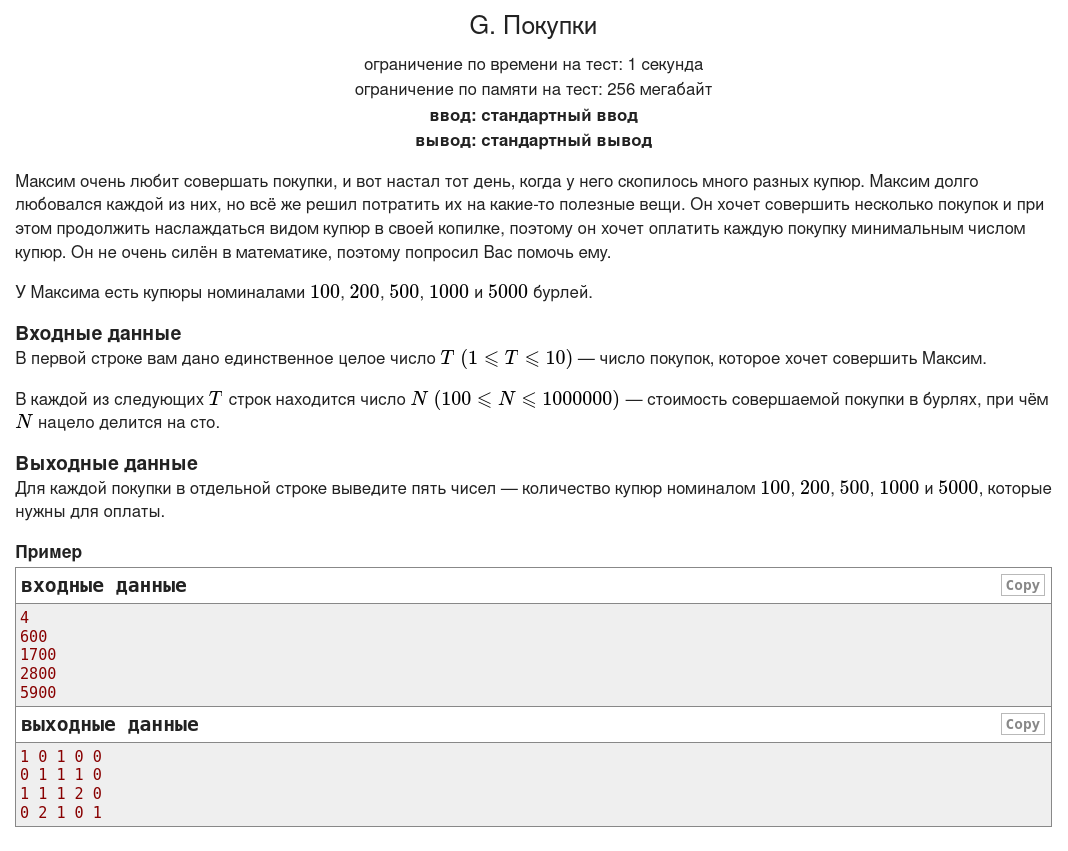
\includegraphics[width=\textwidth]{statements/20220630/G.png}
\end{center}
\subsubsection*{Идея решения}

Идея задачи довольно проста: чтобы в итоге получить минимальное кол-во купюр, необходимо начать с купюр наибольшего достоинства, постепенно переходя к меньшим. Для каждой купюры мы нацело делим оставшуюся сумму денег на её достоинство, получая нужное кол-во купюр. Затем присваиваем переменной $n$ (текущей сумме бурлей) остаток от деления. Для хранения ответа используем вектор размера $5$. Решение работает за $O(t)$, где $t$ --- кол-во тестов (начальных сумм денег) во входных данных (так как кол-во различных купюр фиксировано и равно $5$).

\subsubsection*{Исходный код}
\lstinputlisting{src/20220630/G.cpp}

\subsubsection*{Фрагмент турнирной таблицы контеста}
\begin{center}
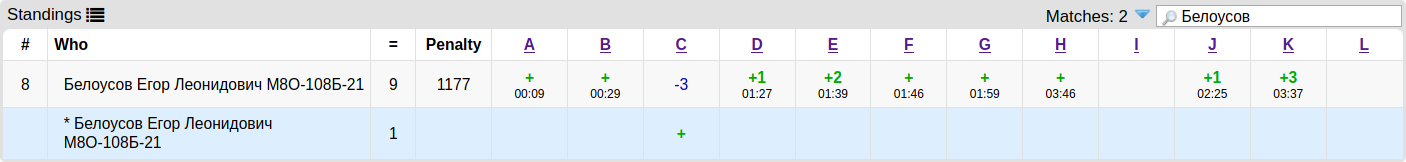
\includegraphics[width=\textwidth]{standings/20220630/table.png}\newline\noindent
\end{center}

\subsubsection*{Выводы}

Задача решена, зачтена чекером с первого раза.

\pagebreak

\subsection*{Библиотека С++}
\begin{center}
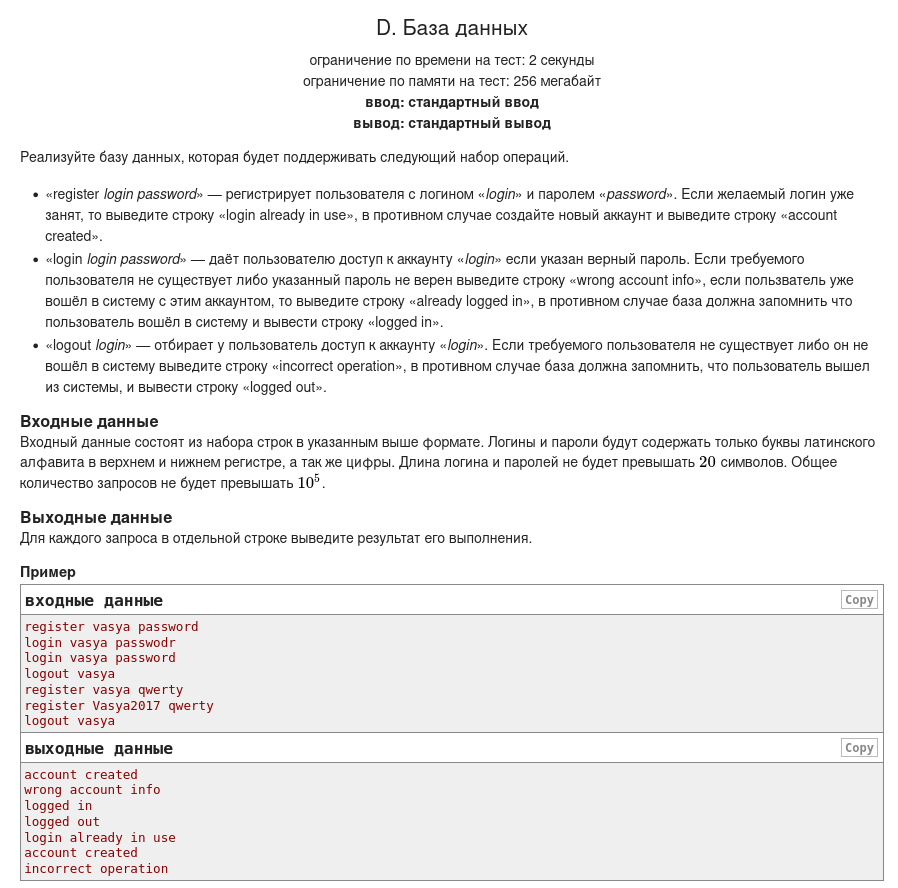
\includegraphics[width=\textwidth]{statements/20220701/D.png}
\end{center}
\subsubsection*{Идея решения}

Интересная задача, позволяющая попрактиковать ООП. Создадим класс $Database$, единственным полем которого будет ассоциативный массив $data$. Ключами в массиве будут логины пользователей, а значениями --- пары, состоящие из пароля и булевского значения "вошёл ли в систему пользователь". Реализуем три метода в классе $Database$: для регистрации нового пользователя, входа и выхода из системы. Осталось дописать в main'е код для считывания команд из условия задачи.

\subsubsection*{Исходный код}
\lstinputlisting{src/20220701/D.cpp}

\subsubsection*{Фрагмент турнирной таблицы контеста}
\begin{center}
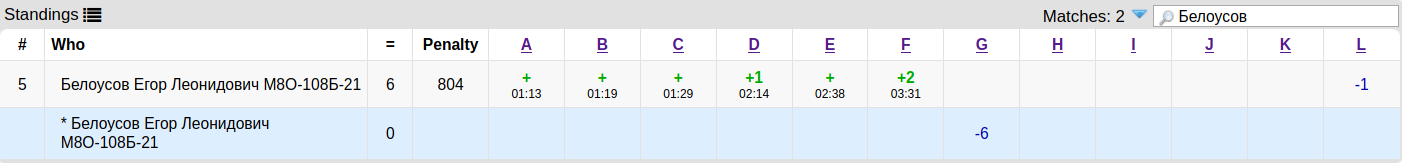
\includegraphics[width=\textwidth]{standings/20220701/table.png}\newline\noindent
\end{center}

\subsubsection*{Выводы}

Задача решена, зачтена чекером со второго раза, вначале забыл дописать перенос строки в выходных данных.

\pagebreak

\subsection*{Динамическое программирование}
\begin{center}
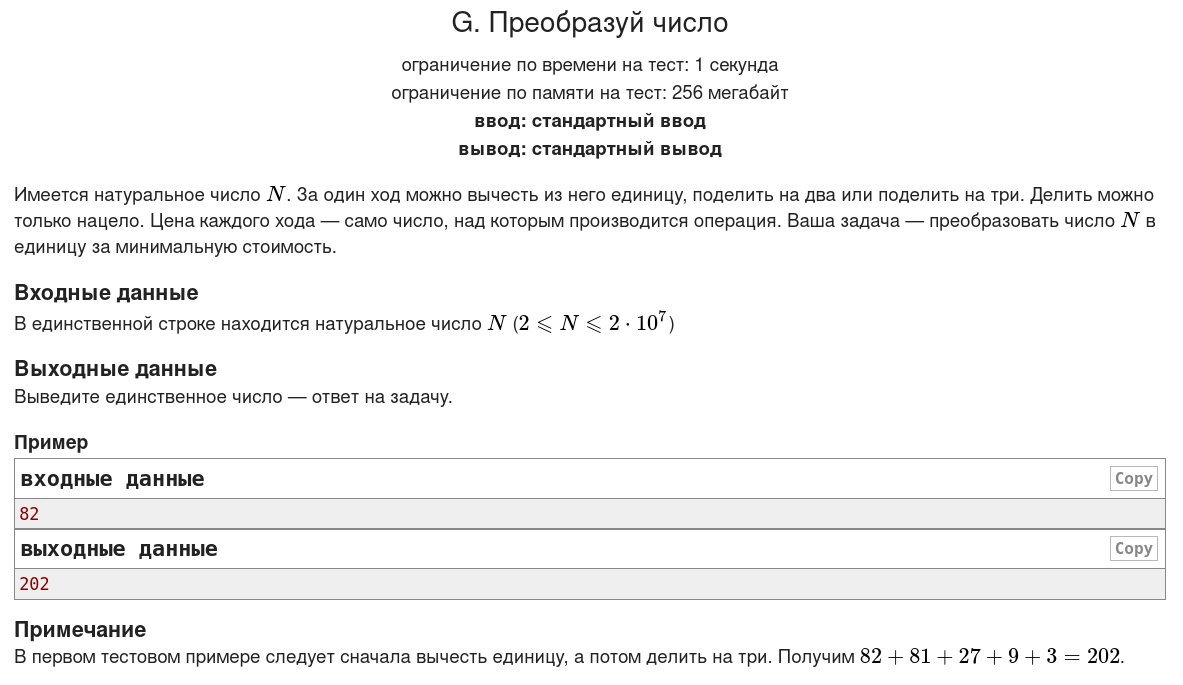
\includegraphics[width=\textwidth]{statements/20220702/G.png}
\end{center}
\subsubsection*{Идея решения}

Одна из классических задач на динамическое программирование. В условии нас просят преобразовать число $n$ в единицу, мы же пойдем "с конца"{}, то есть, от единицы к самому числу. Изначально (в единице) стоимость операций равна нулю, т.к. нам не нужно из единицы делать единицу. Заведём вектор $dp$ размера $n + 1$, заполним его константой $INF$, большей любого возможного числа $n$. $dp[i]$ --- минимальная стоимость преобразования числа $i$ в единицу. Обозначим $dp[1] = 0$. При этом для всех $i > 1$ должно выполняться $dp[i] = i + min(dp[i - 1], dp[i / 2], dp[i / 3])$, т.е. мы приходим в число $i$ либо из предыдущего числа $i - 1$, либо из чисел $i / 2$, $i / 3$ (если $i$ нацело делится на $2$ или $3$). Заполняем массив $dp$ в цикле от $2$ до $n$ включительно. Ответ на задачу --- число $dp[n]$. Алгоритм работает за $O(n)$, т.е. за линейное время.

\subsubsection*{Исходный код}
\lstinputlisting{src/20220702/G.cpp}

\subsubsection*{Фрагмент турнирной таблицы контеста}
\begin{center}
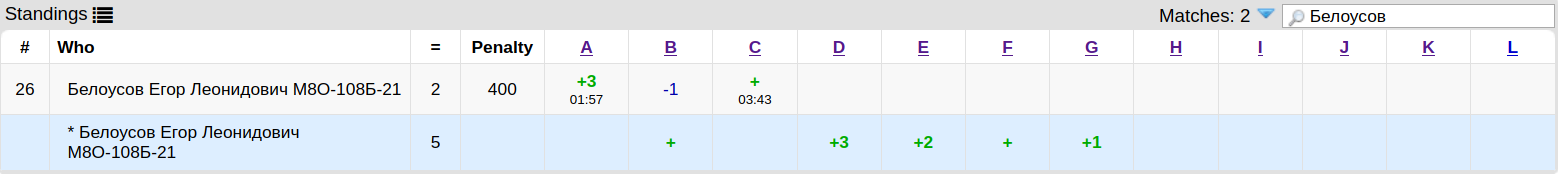
\includegraphics[width=\textwidth]{standings/20220702/table.png}\newline\noindent
\end{center}

\subsubsection*{Выводы}

Задача дорешана, зачтена чекером со второго раза (поправил константу $INF$ и размер массива $dp$).

\pagebreak

\subsection*{Префиксные суммы, сортировка событий, два указателя}
\begin{center}
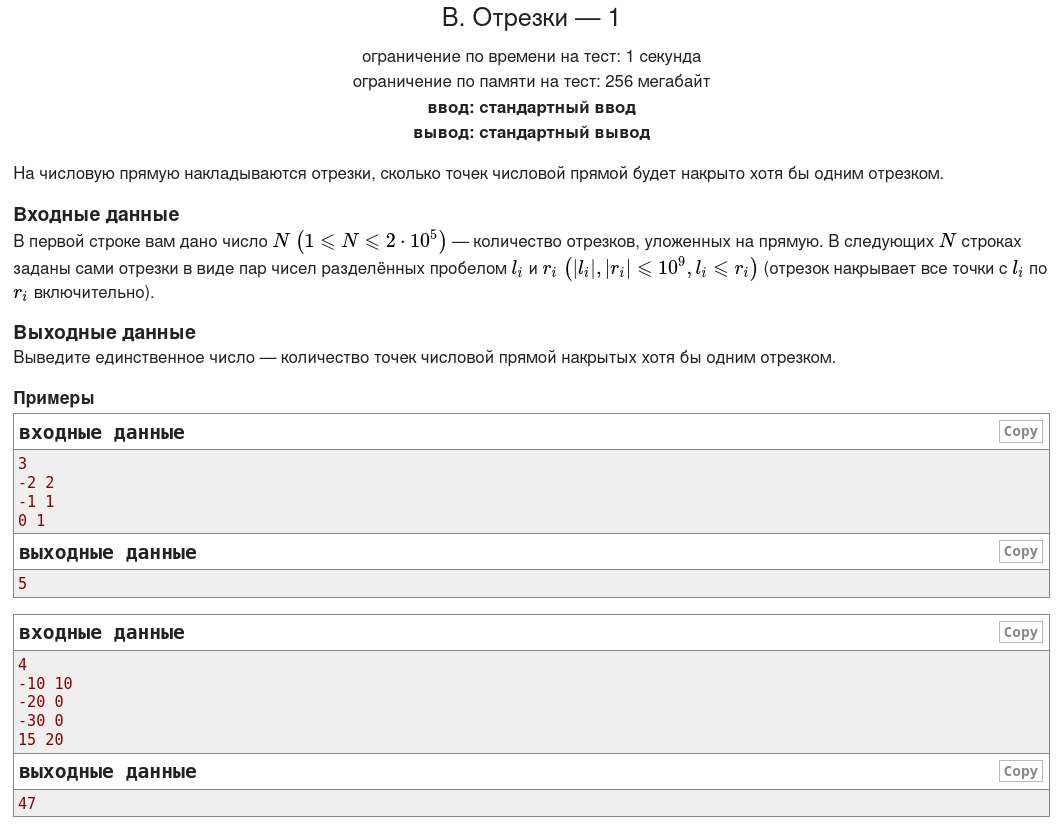
\includegraphics[width=\textwidth]{statements/20220704/B.png}
\end{center}
\subsubsection*{Идея решения}

Представим входные данные (границы отрезков) в виде двух событий: начала и конца отрезка. Каждое событие зададим парой чисел $(i, event)$, где $i$ --- индекс события на числовой прямой, $event$ --- код события ($1$ --- начало отрезка, $2$ --- его конец). Причём для конца отрезка индекс будет на единицу больше, т.к. крайняя правая точка отрезка всё ещё входит в этот самый отрезок, а точка на единицу правее --- уже нет. Отсортируем массив событий, и далее, идя по нему в цикле, будем с помощью переменной $cnt$ фиксировать, сколько отрезков покрывает текущую точку (и все точки до предыдущего события). Таким образом, вместо того, чтобы идти по всей числовой прямой, границы которой по условию от $-10^9$ до $10^9$, или, например, по всем точкам внутри отрезков, мы рассматриваем лишь начало и конец каждого отрезка. Сложность алгоритма --- $O(2*n) == O(n)$, где $n$ --- кол-во отрезков.

\subsubsection*{Исходный код}
\lstinputlisting{src/20220704/B.cpp}

\subsubsection*{Фрагмент турнирной таблицы контеста}
\begin{center}
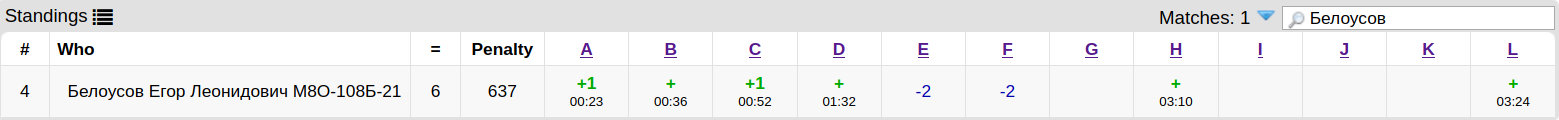
\includegraphics[width=\textwidth]{standings/20220704/table.png}\newline\noindent
\end{center}

\subsubsection*{Выводы}

Задача решена, зачтена чекером с первого раза.

\pagebreak

\subsection*{ДП, задача о рюкзаке}
\begin{center}
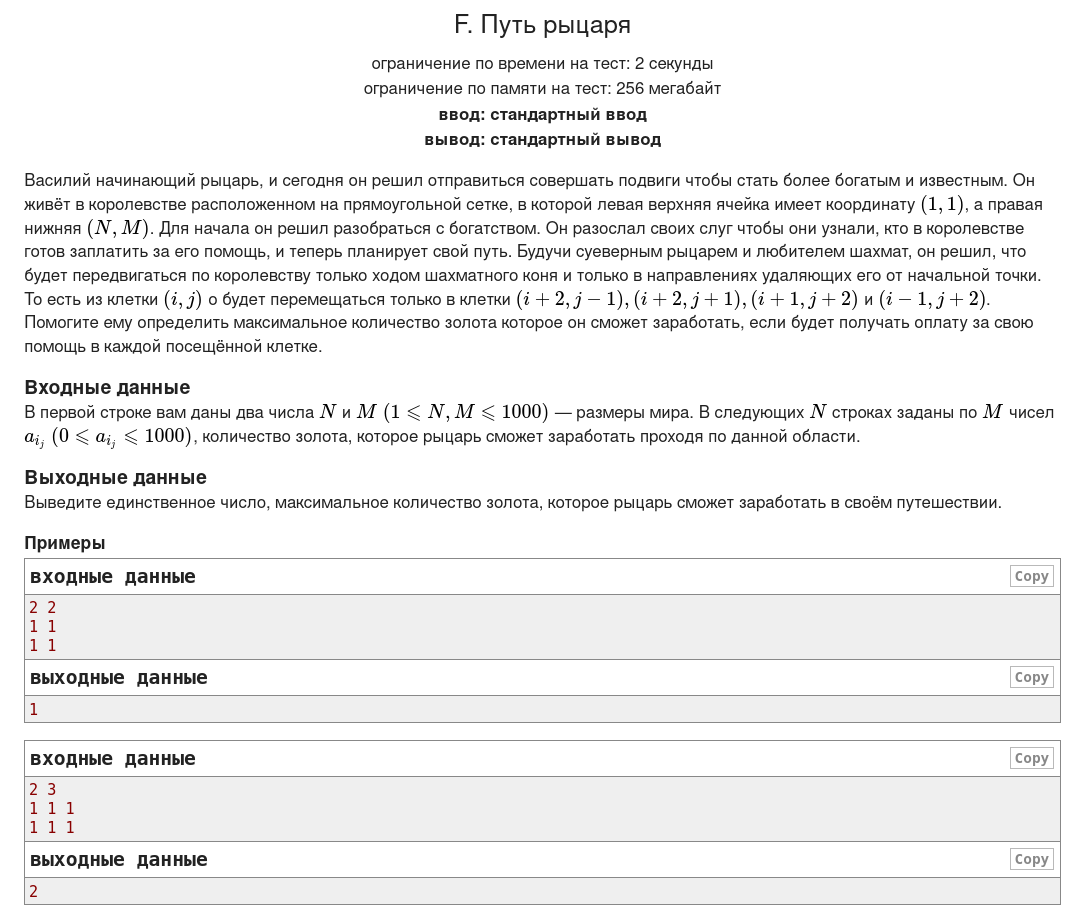
\includegraphics[width=\textwidth]{statements/20220705/F1.png}
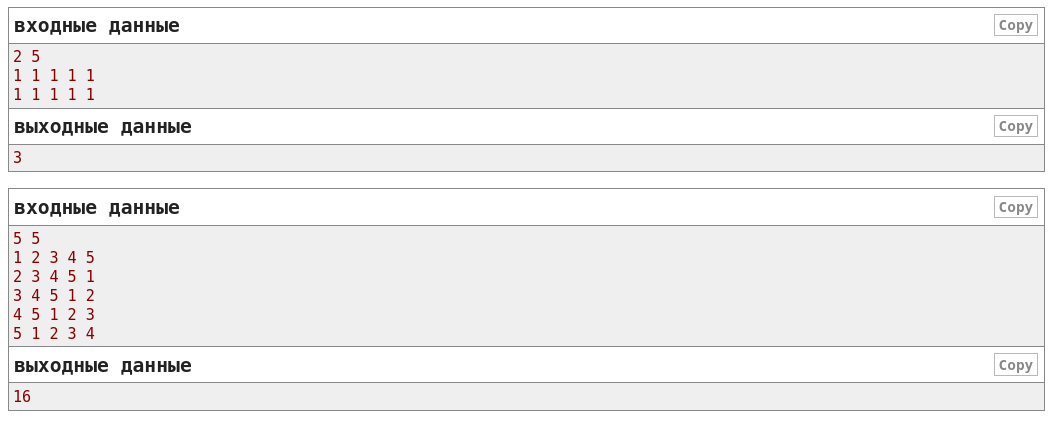
\includegraphics[width=\textwidth]{statements/20220705/F2.png}
\end{center}
\subsubsection*{Идея решения}

Наиболее трудным шагом в решении было понять, каким образом осуществлять обход поля, т.е. как построить динамику. Я пришёл к выводу, что неплохим вариантом будет идти по диагоналям, т.к. ход конём подразумевает, что нам в точке $(i, j)$ должны быть известны предыдущие данные с точек $(i - 2, j + 1)$, $(i - 2, j - 1)$, $(i - 1, j - 2)$, $(i + 1, j - 2)$. Проблему разных размеров диагоналей в прямоугольниках разных размеров (неудобно обходить диагонали) я решил, выделив в отдельную функцию $get\_indexes$ получение нужного вектора точек обхода. Функция $get\_dp$, получая на вход очередную точку $(i, j)$, возвращает $dp[i][j]$ --- максимальное число золота, которое можно получить, попав в точку $(i, j)$. Из доступных предыдущих точек (индексы которых не выходят за границы поля) берётся максимум, и добавляется значение золота в текущей точке $(i, j)$. Ответом является максимальное значение $dp[i][j]$ для любых $i$, $j$. Алгоритм работает за $O((max(n, m))^2)$, т.к. внешний цикл идёт до $n + m - 1$, внутренний --- до текущего значения счётчика внешнего цикла $k$: $1 + 2 + ... + (n + m - 1) = ((n + m - 1) * (n + m)) / 2$.

\subsubsection*{Исходный код}
\lstinputlisting{src/20220705/F.cpp}

\subsubsection*{Фрагмент турнирной таблицы контеста}
\begin{center}
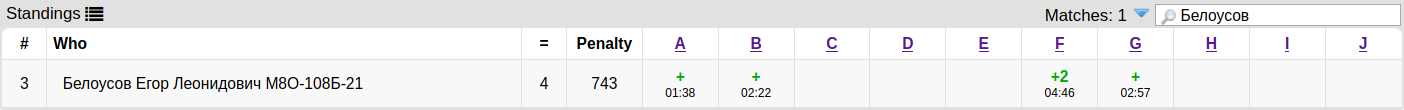
\includegraphics[width=\textwidth]{standings/20220705/table.png}\newline\noindent
\end{center}

\subsubsection*{Выводы}

Задача решена, зачтена чекером с третьего раза (поправил мелкие недочёты: $<=$ вместо $<$, объявление переменной $res = -1$ вместо $res = 0$).

\pagebreak

\subsection*{Длинная арифметика}
\begin{center}
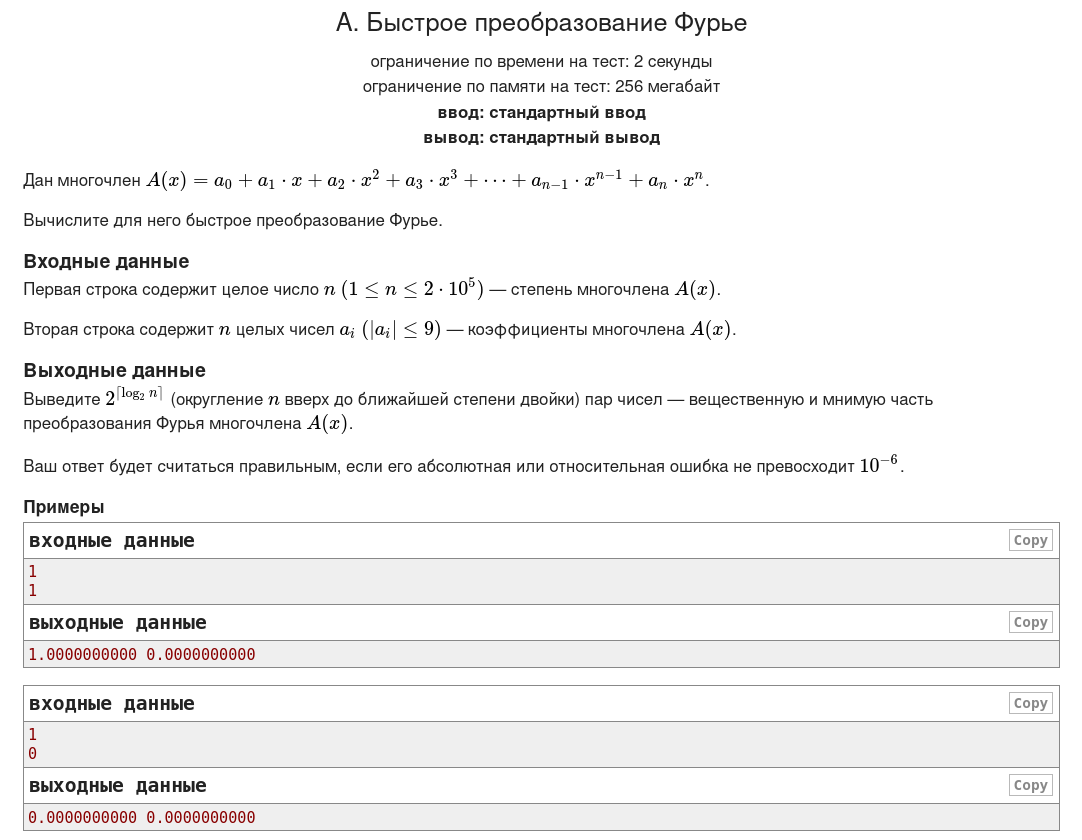
\includegraphics[width=\textwidth]{statements/20220706/A1.png}
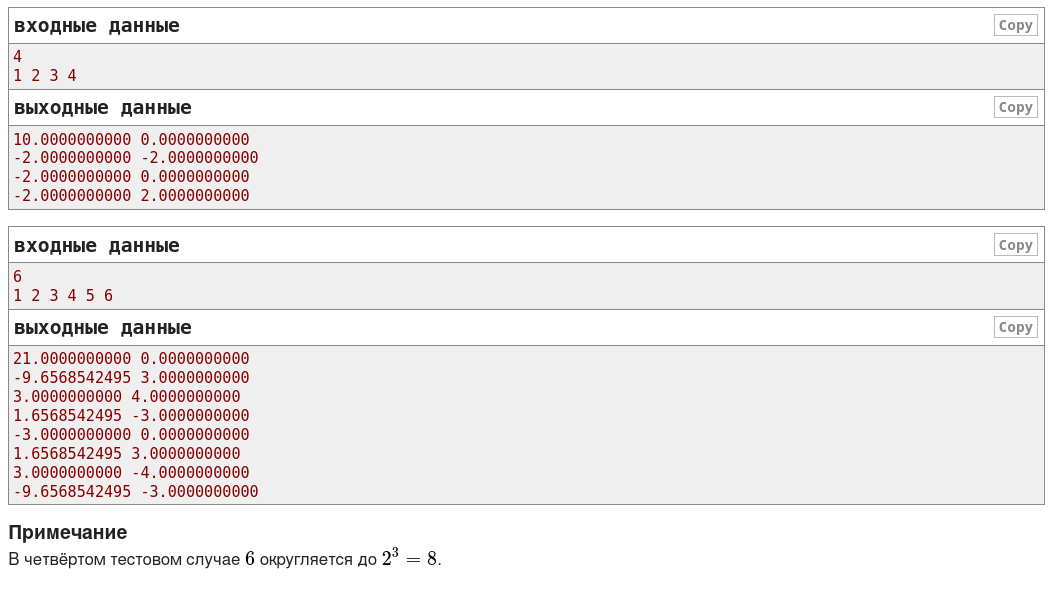
\includegraphics[width=\textwidth]{statements/20220706/A2.png}
\end{center}
\subsubsection*{Идея решения}

Быстрым пребразованием Фурье (БПФ, FFT) называется алгоритм вычисления дискретного преобразования Фурье (ДПФ), позволяющий найти его коэффициенты за $O(n*log(n))$, что существенно быстрее по сравнению с вычислением напрямую, по формуле, за $O(n^2)$. Чтобы ускорить вычисления, применяется принцип "разделяй-и-властвуй"{}, по которому коэффициенты исходного многочлена разбиваются на две группы: чётные и нечётные. От каждой группы считается DFT, и в результате находится DFT исходного многочлена. Используя свойства коэффициентов преобразования Фурье, мы сводим задачу к двум подзадачам вдвое меньшего размера.

\subsubsection*{Исходный код}
\lstinputlisting{src/20220706/A.cpp}

\subsubsection*{Фрагмент турнирной таблицы контеста}
\begin{center}
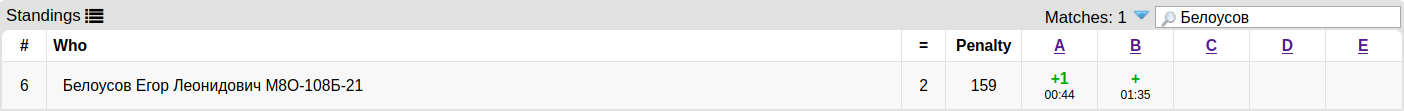
\includegraphics[width=\textwidth]{standings/20220706/table.png}\newline\noindent
\end{center}

\subsubsection*{Выводы}

Задача решена, зачтена чекером с третьего раза (исправил ошибку с числом пи, поправил точность вывода).

\pagebreak

\subsection*{Основы теории графов}
\begin{center}
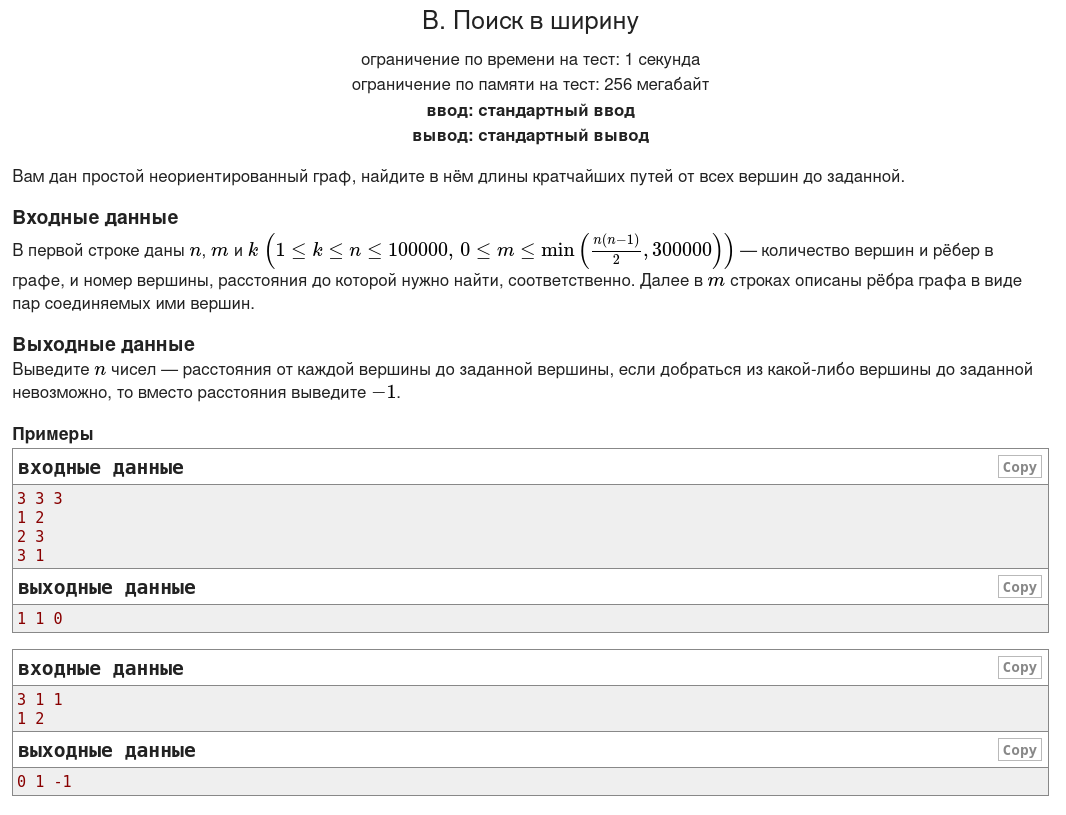
\includegraphics[width=\textwidth]{statements/20220707/B.png}
\end{center}
\subsubsection*{Идея решения}

Поиск в ширину (BFS, breadth-first search) является одним из методов обхода графа. Он работает, перебирая все вершины, выходящие из текущей, и добавляя их в очередь (queue). Далее для каждой вершины в очереди процесс повторяется, и так далее. Таким образом, граф делится на определённые "уровни"{}, т.е. минимальные расстояния от исходной вершины до любой другой в графе. Сложность --- $O(n + m)$, где $n$ --- кол-во вершин в графе, а $m$ --- кол-во рёбер.

\subsubsection*{Исходный код}
\lstinputlisting{src/20220707/B.cpp}

\subsubsection*{Фрагмент турнирной таблицы контеста}
\begin{center}
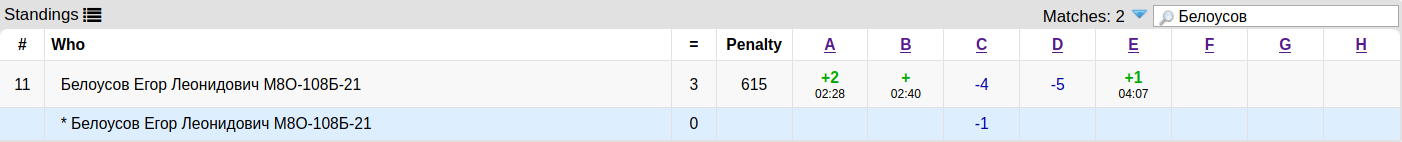
\includegraphics[width=\textwidth]{standings/20220707/table.png}\newline\noindent
\end{center}

\subsubsection*{Выводы}

Задача решена, зачтена чекером с первого раза.

\pagebreak

\subsection*{Кратчайшие пути во взвешенных графах}
\begin{center}
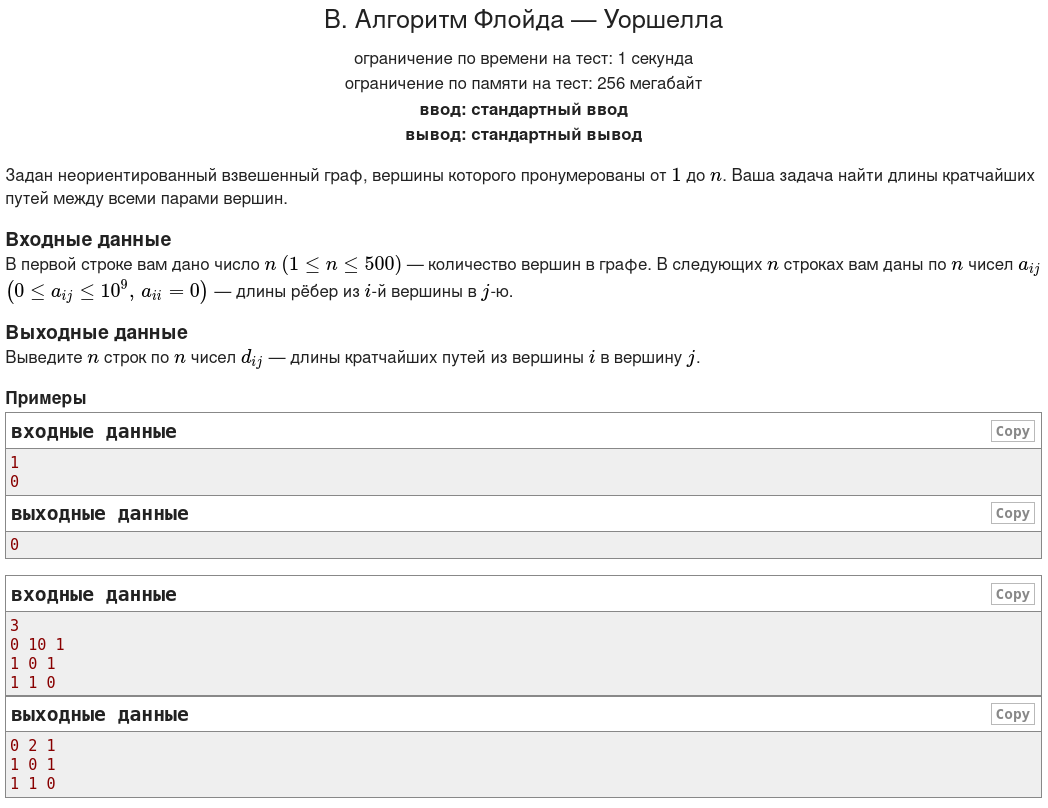
\includegraphics[width=\textwidth]{statements/20220708/B.png}
\end{center}
\subsubsection*{Идея решения}

Алгоритм Флойда-Уоршелла --- это алгоритм поиска кратчайших путей во взвешенном графе, в котором могут быть рёбра как с положительным, так и с отрицательным весом (но не должно быть отрицательных циклов). Он работает за $O(n^3)$, где $n$ --- число вершин в графе, и основывается на ограничении понятия кратчайшего пути из $u$ в $v$ множеством $\{1..i\}$. Обозначим $d_{uv}^{(i)}$ длину кратчайшего пути из вершины $u$ в вершину $v$, содержащего, кроме начала и конца, только вершины из мн-ва $\{1..i\}$. При этом $d_{uv}^{(0)}$ равно длине ребра между $u$ и $v$, если оно существует в графе, и $\infty$, если нет. На каждом шаге алгоритма будем брать очередную вершину и для всех пар $u$ и $v$ вычислять значение $d_{uv}^{(i)} = min(d_{uv}^{(i-1)}, d_{ui}^{(i-1)} + d_{iv}^{(i-1)})$. Эта формула говорит о том, что если вершина $i$ содержится в кратчайшем пути из $u$ в $v$, то таким путём является путь из $u$ в $i$, объединённый с путём из $i$ в $v$. Иначе, таким путём является кратчайший путь из $u$ в $v$, содержащий лишь вершины из мн-ва $\{1..i-1\}$.

\subsubsection*{Исходный код}
\lstinputlisting{src/20220708/B.cpp}

\subsubsection*{Фрагмент турнирной таблицы контеста}
\begin{center}
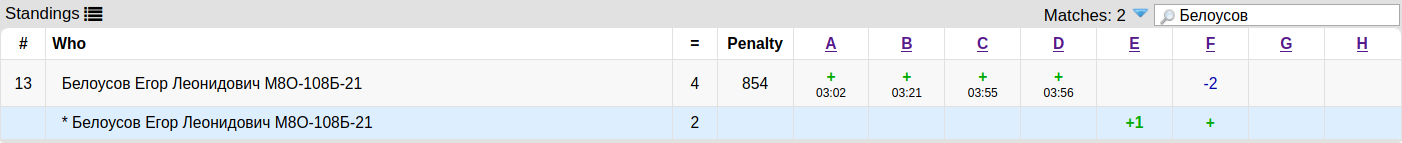
\includegraphics[width=\textwidth]{standings/20220708/table.png}\newline\noindent
\end{center}

\subsubsection*{Выводы}

Задача решена, зачтена чекером с первого раза.

\pagebreak

\subsection*{Алгоритмы на строках}
\begin{center}
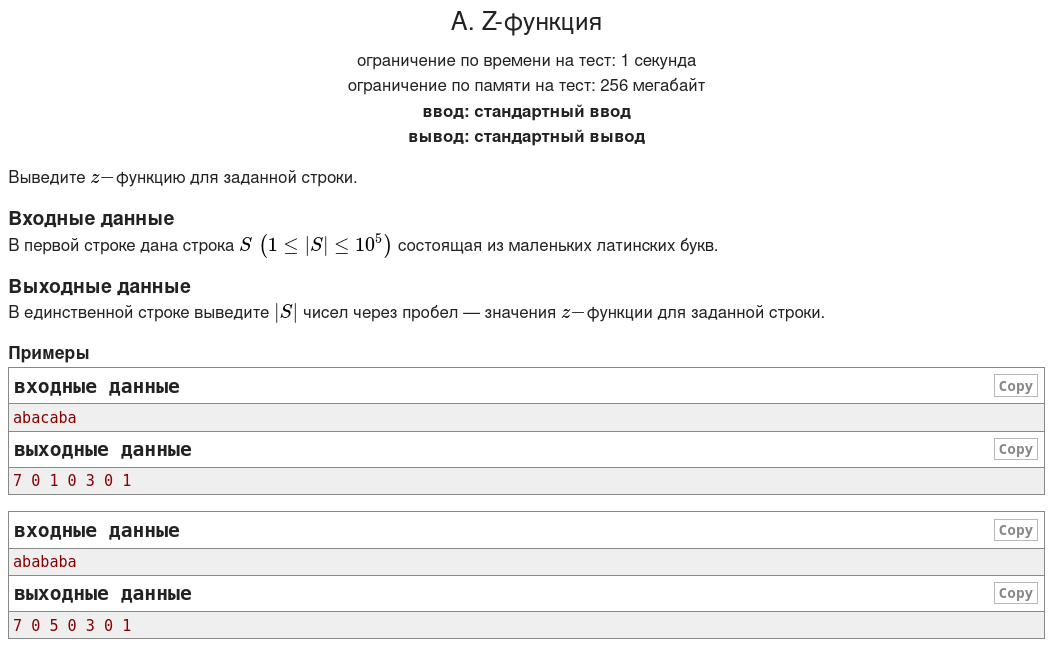
\includegraphics[width=\textwidth]{statements/20220709/A.png}
\end{center}
\subsubsection*{Идея решения}

$Z$--функцией строки $S$ и позиции $x$ называется длина максимального префикса подстроки, начинающейся с позиции $x$ в строке $S$, который одновременно является и префиксом всей строки $S$. Значение $Z$--функции от первого символа в строке не определено, поэтому его обычно приравнивают либо к длине строки, либо к нулю. Существует тривиальный алгоритм поиска $Z$--функции, работающий за $O(n^2)$, где $n$ --- длина строки. Он представляет собой простой перебор всех индексов и префиксов с нахождением максимального для каждого индекса. Более эффективный алгоритм работает за $O(n)$ и представлен в решении этой задачи. Обозначим $l$ и $r$ --- границы самого правого отрезка совпадения, причём $r$ в отрезок не входит, т.е. $s[l, r) = s[0, z[i])$. Изначально $l = r = 0$. Пусть известны значения $Z$--функции от $0$ до $i - 1$. Найдём $z[i]$. Рассмотрим 2 случая:
\begin{itemize}
 \setlength{\itemindent}{1em}
  \item[$1.$] $i > r$:\\
  В этом случае просто "наивно"{} пробегаемся по строке $S$, сравнивая символы в позициях $s[i + j]$ и $s[j]$. Первая такая позиция $j$, для которой не выполняется $s[i + j] = s[j]$, и является значением $z[i]$.
  \item[$2.$] $i <= r$:\\
  Сравним $z[i - l] + i$ и $r$. Если $r$ меньше, то "наивно"{} пробегаемся по строке, начиная с $r$, и вычисляем $z[i]$. В противном случае нам уже известно значение $z[i]$, равное $z[i - l]$.
\end{itemize}

\subsubsection*{Исходный код}
\lstinputlisting{src/20220709/A.cpp}

\subsubsection*{Фрагмент турнирной таблицы контеста}
\begin{center}
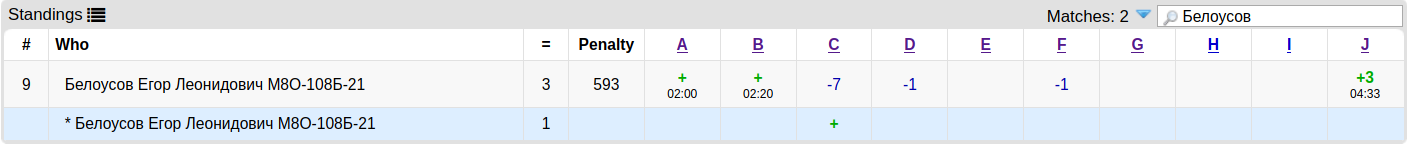
\includegraphics[width=\textwidth]{standings/20220709/table.png}\newline\noindent
\end{center}

\subsubsection*{Выводы}

Задача решена, зачтена чекером с первого раза.

\pagebreak
